\documentclass{article}
\usepackage{graphicx}
\usepackage{float}
\usepackage[margin=.75in]{geometry}

\usepackage{hyperref}
\hypersetup{
    colorlinks=true,
    linkcolor=blue,
    filecolor=magenta,      
    urlcolor=cyan,
}
 
\urlstyle{same}
\begin{document}

Code used in production of plots for this section can be found at https://github.com/cfmcginn/SystBio/tree/master/HW8.
\section{2.c}

\begin{figure}[H]
    \centering
    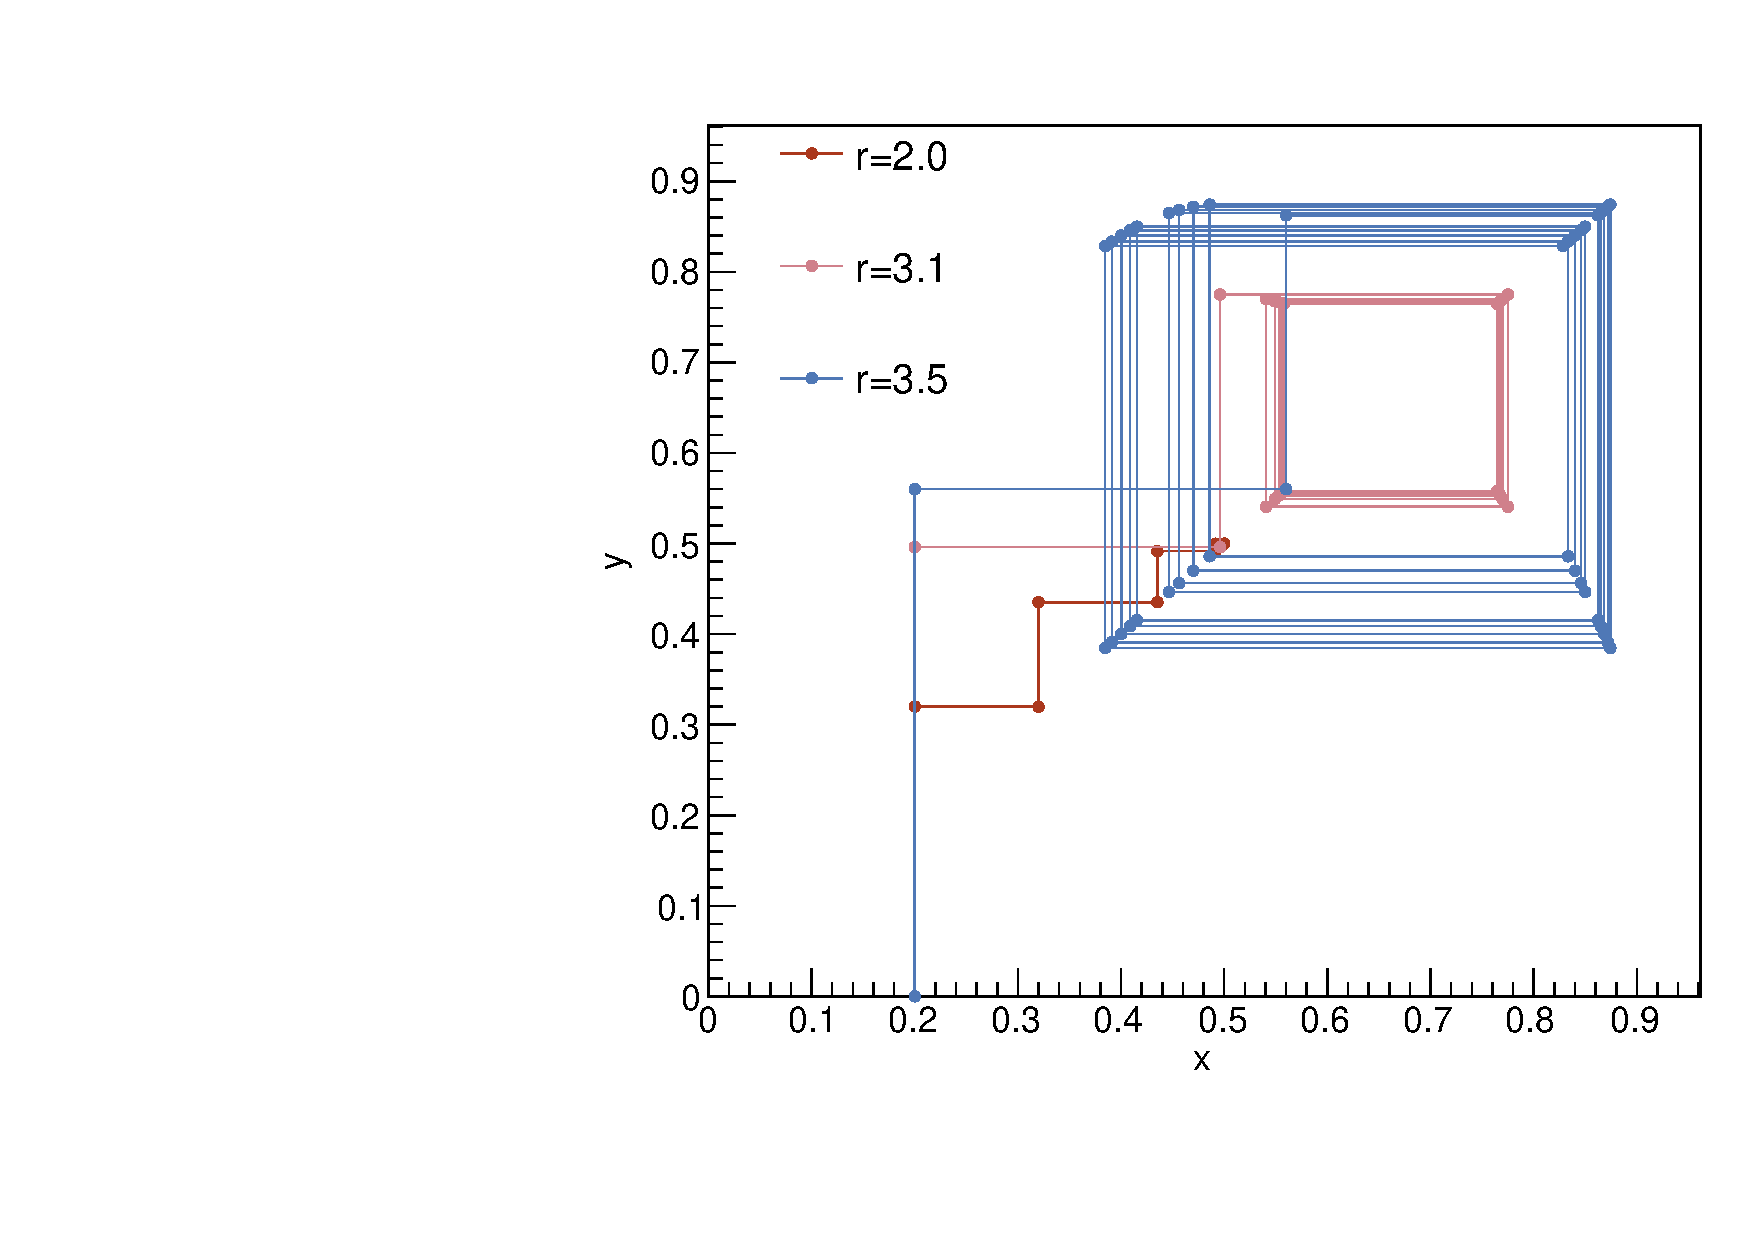
\includegraphics[width=.45\textwidth]{cobWeb.pdf} 
    \caption{Cobweb diagram for R = 2, R = 3.1, and R = 3.5 (see legend). R=2 approaches a final value in a regular fashion, whille other R values oscillate}
    \label{fig:fig1}
\end{figure}

In Fig.~\ref{fig:fig1} we see that R of 2 approaches a final value in a regularized way, while R of 3.1 and 3.5 go through cycles of values. This is consistent with the qualitative checks  of b and c. Of the two cycling cobwebs, the larger r parameter (3.5) has a larger area cycle than smaller r.

\section{2.d}

\begin{figure}[H]
    \centering
    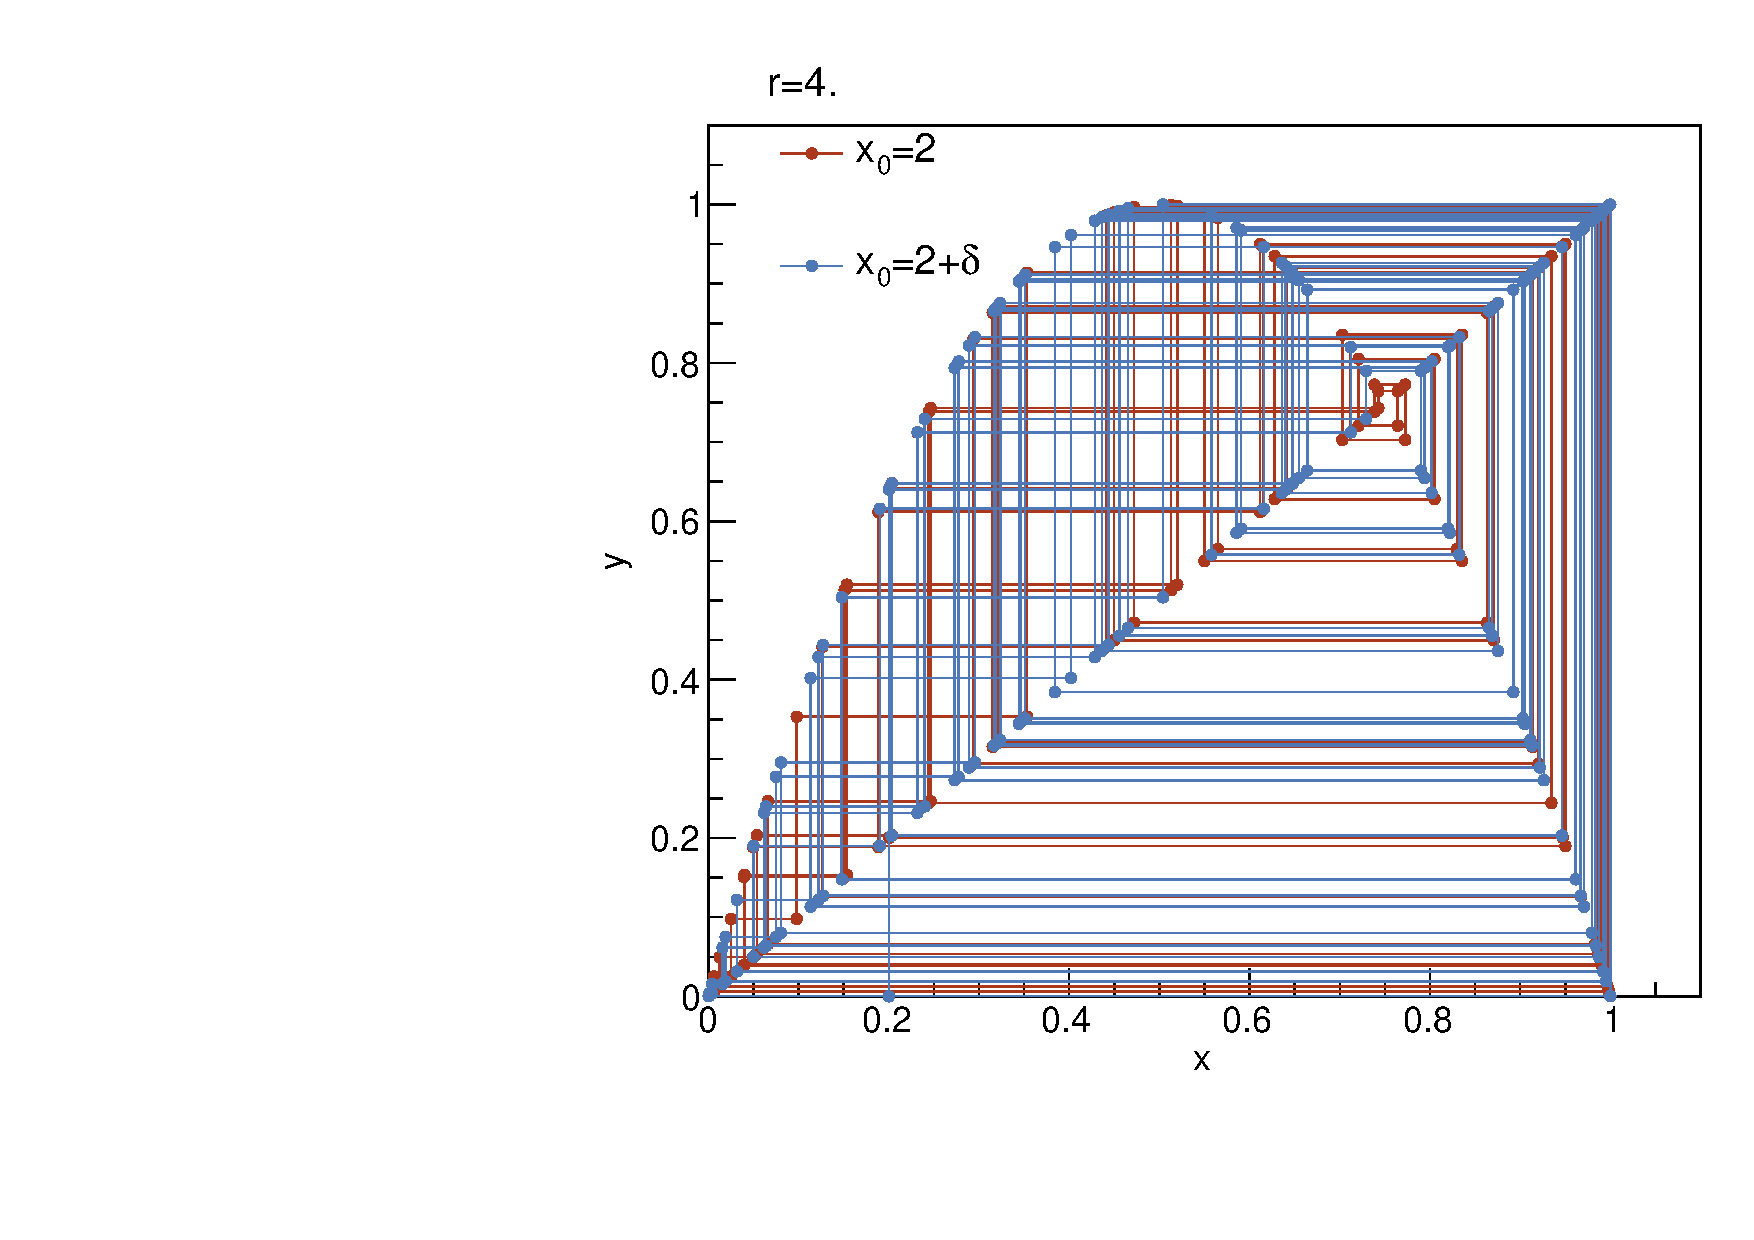
\includegraphics[width=.45\textwidth]{cobWeb2.pdf} 
    \caption{Cobweb diagram for r=4. of the logistic map w/ initial conditions of 2. and 2.00000001. Shown here is how small perturbations in initial condition for this logistic map can lead to very different long term behavior, or chaos.}
    \label{fig2}
\end{figure}

\begin{figure}[H]
    \centering
    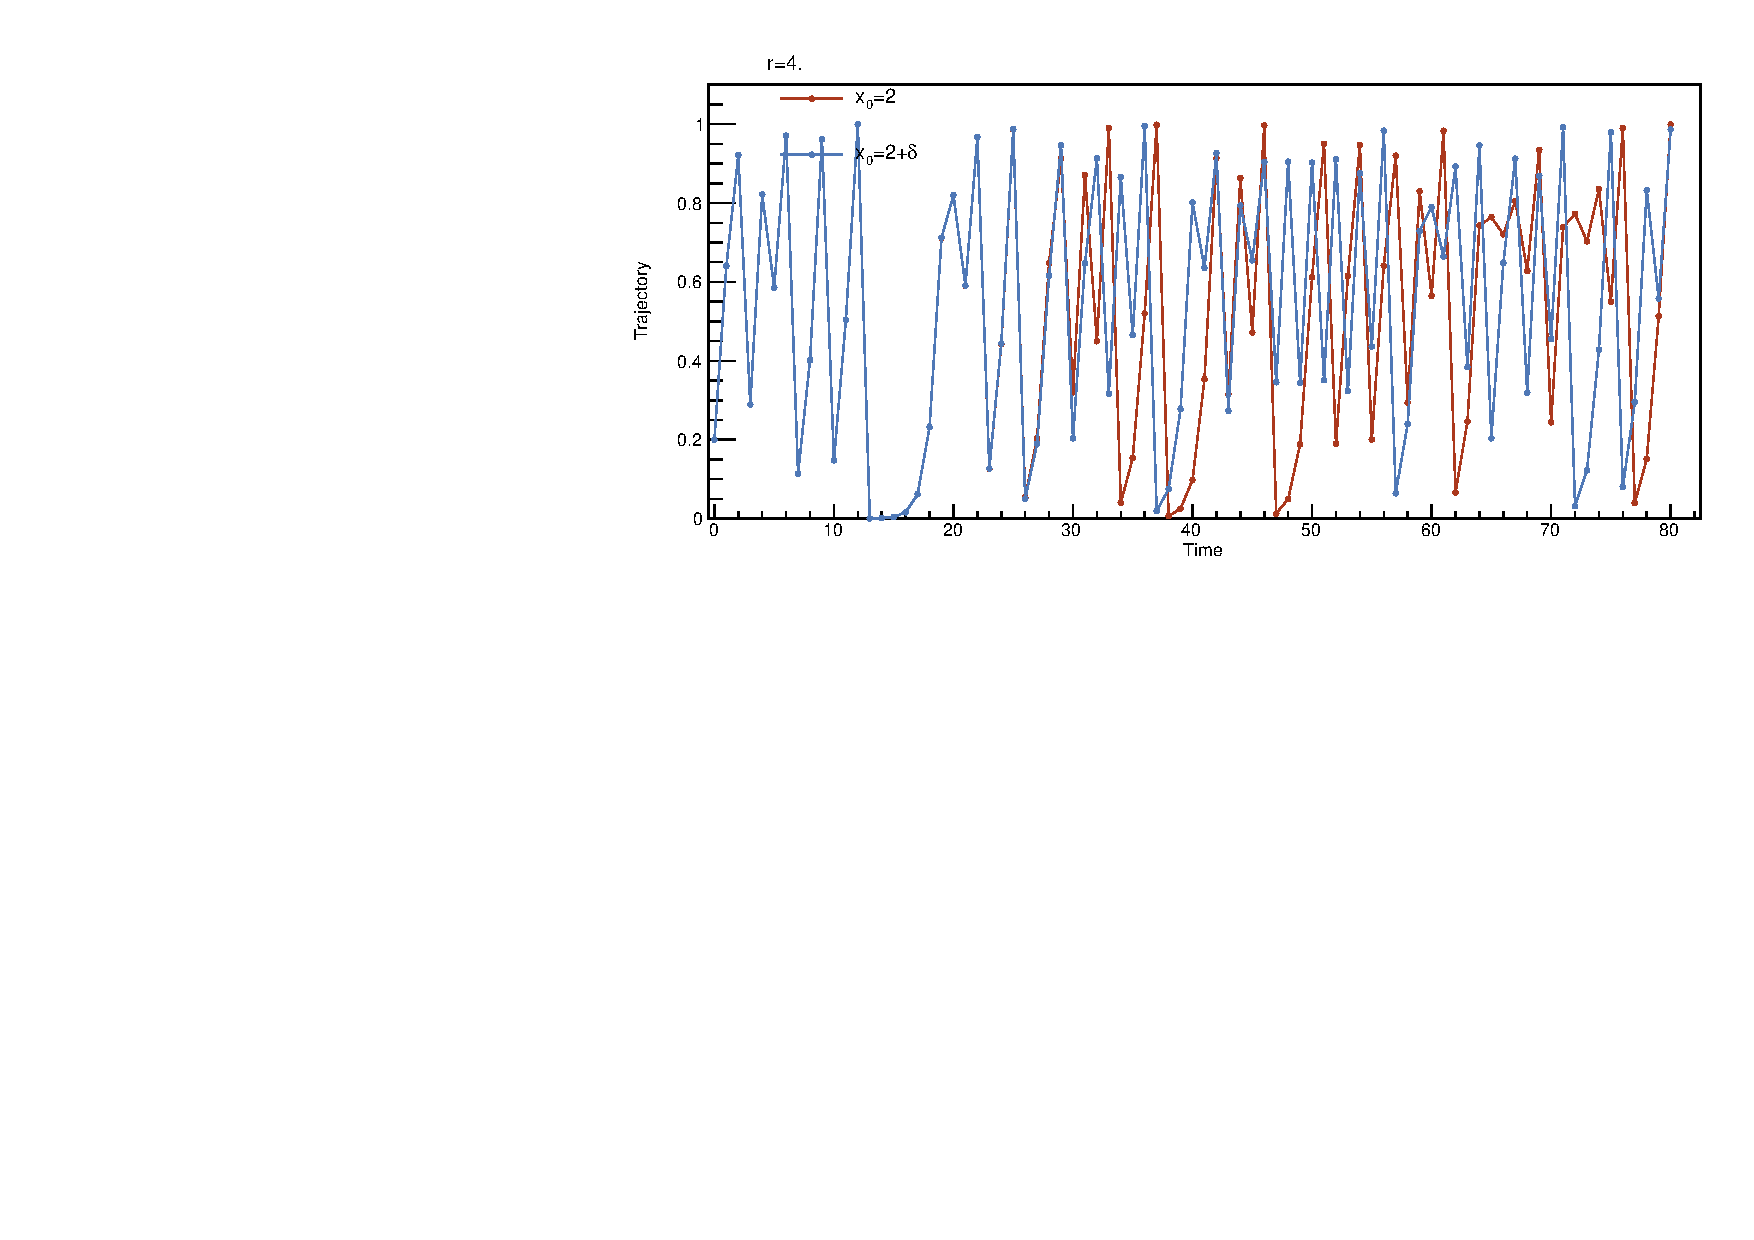
\includegraphics[width=.8\textwidth]{traj_79.pdf} 
    \caption{Time trajectory of logistic map of identical r parameter 4 but differing initial conditions (by some small delta as given in the problem). Clearly for long time steps we get very different behavior for the two initial conditions despite their small separation.}
    \label{fig3}
\end{figure}

\begin{figure}[H]
    \centering
    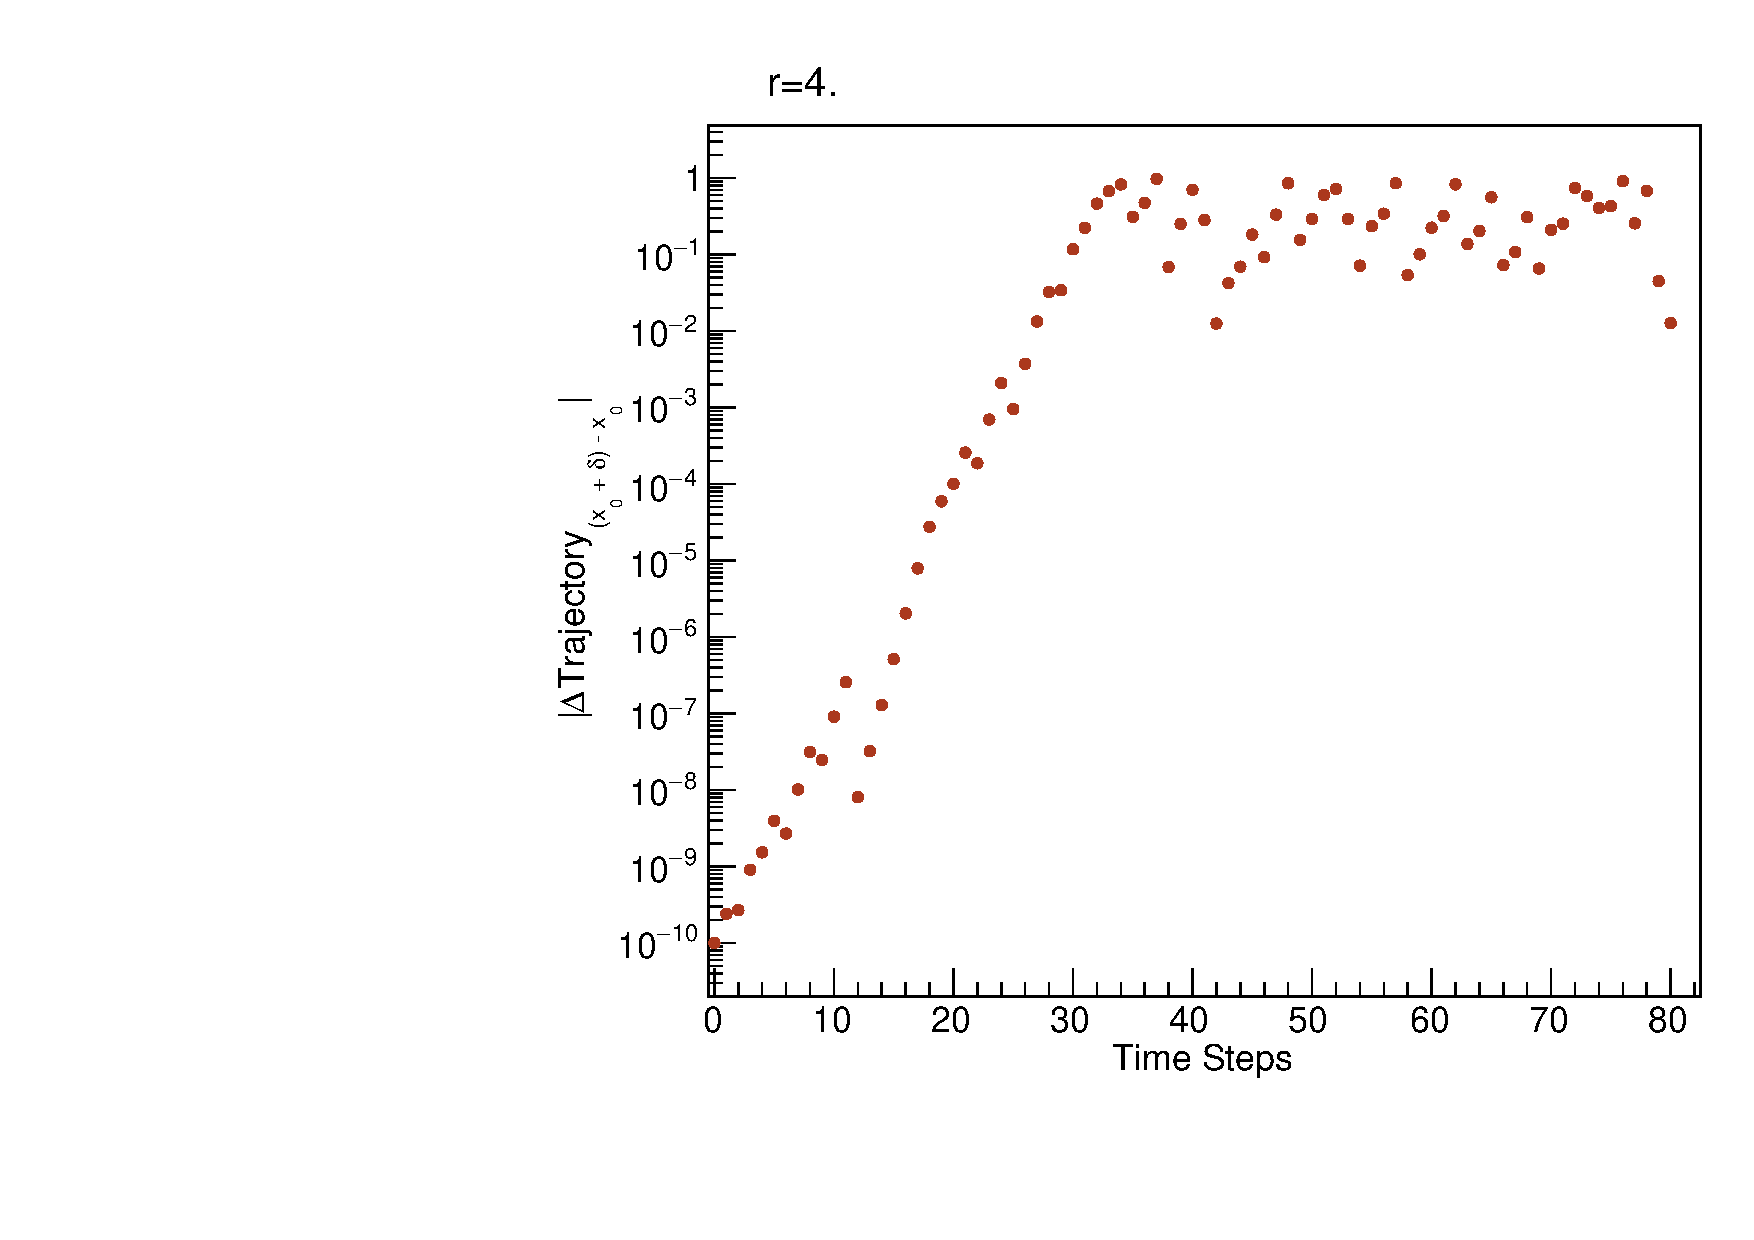
\includegraphics[width=.45\textwidth]{deltaTraj.pdf} 
    \caption{Difference in the trajectories of identical logistic map equation with differing initial condition. Trajectory difference increases multiple orders of magnitude over the first 30 time steps before settling into oscillations between .1 and 1 for the remaining 50 time steps.}
    \label{fig4}
\end{figure}

In Figures ~\ref{fig2}-~\ref{fig3} we see that for identical logistical maps with r=4 with initial conditions differing by some infinitesimal delta we get very different behavior on long time scales. Clearly the long term behavior of the logistical map in this parameter space is highly sensitive to initial conditions. From Fig.~\ref{fig4}, the trajectory is initially linear on a log-y scale, implying power law dependence. It eventually settles into oscillations between .1 and 1 for time steps greater than 30.


For a cobweb gif of chaos, see link here: \href{https://github.com/cfmcginn/SystBio/blob/master/HW8/fullChaos.gif}{https://github.com/cfmcginn/SystBio/blob/master/HW8/fullChaos.gif}.

For a time plot gif of chaos, see link here: \href{https://github.com/cfmcginn/SystBio/blob/master/HW8/traj.gif}{https://github.com/cfmcginn/SystBio/blob/master/HW8/traj.gif}.


\end{document}

